\section{Audio Spectrograms}
\subsection{Disclaimer}
I want to start with the disclaimer that I do not study EE and that
prior to starting this project for COMP4121 I had no knowledge of digital signal processing.
The only things I knew before were from doing music production as a hobby.
In short, some of this report may be misinformation. Have fun reading!

\subsection{Audio signals}
An discrete signal $x$ is a sequence of real valued samples $(\dots, x[-1], x[0], x[1], x[2], \dots)$.
These real numbers correspond to the voltage that would be held across a speaker at each point in time.
The number of samples per second of audio is known as the \emph{sampling rate}.
\begin{center}

\tikzset{every picture/.style={line width=0.75pt}} %set default line width to 0.75pt        

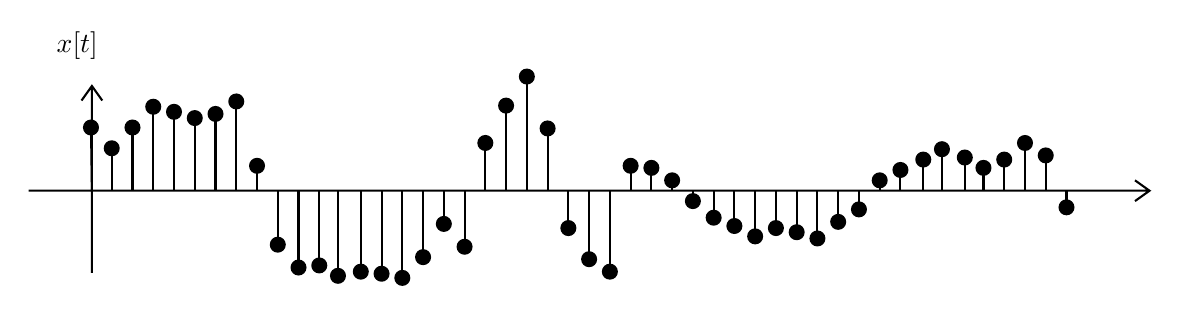
\begin{tikzpicture}[x=0.75pt,y=0.75pt,yscale=-1,xscale=1]
%uncomment if require: \path (0,300); %set diagram left start at 0, and has height of 300

%Shape: Axis 2D [id:dp21174656794965774] 
\draw  (30,130.45) -- (570,130.45)(60.45,80) -- (60.45,170) (563,125.45) -- (570,130.45) -- (563,135.45) (55.45,87) -- (60.45,80) -- (65.45,87)  ;
%Straight Lines [id:da8619680707928699] 
\draw    (60.45,130.45) -- (60,100) ;
\draw [shift={(60,100)}, rotate = 269.15] [color={rgb, 255:red, 0; green, 0; blue, 0 }  ][fill={rgb, 255:red, 0; green, 0; blue, 0 }  ][line width=0.75]      (0, 0) circle [x radius= 3.35, y radius= 3.35]   ;
%Straight Lines [id:da4766141421180752] 
\draw    (70,130.55) -- (70,110) ;
\draw [shift={(70,110)}, rotate = 270] [color={rgb, 255:red, 0; green, 0; blue, 0 }  ][fill={rgb, 255:red, 0; green, 0; blue, 0 }  ][line width=0.75]      (0, 0) circle [x radius= 3.35, y radius= 3.35]   ;
%Straight Lines [id:da3582398504173244] 
\draw    (80,130.55) -- (80,100) ;
\draw [shift={(80,100)}, rotate = 270] [color={rgb, 255:red, 0; green, 0; blue, 0 }  ][fill={rgb, 255:red, 0; green, 0; blue, 0 }  ][line width=0.75]      (0, 0) circle [x radius= 3.35, y radius= 3.35]   ;
%Straight Lines [id:da5925240937835147] 
\draw    (90,130.55) -- (90,90) ;
\draw [shift={(90,90)}, rotate = 270] [color={rgb, 255:red, 0; green, 0; blue, 0 }  ][fill={rgb, 255:red, 0; green, 0; blue, 0 }  ][line width=0.75]      (0, 0) circle [x radius= 3.35, y radius= 3.35]   ;
%Straight Lines [id:da9324351246162563] 
\draw    (100,130.55) -- (100,92.45) ;
\draw [shift={(100,92.45)}, rotate = 270] [color={rgb, 255:red, 0; green, 0; blue, 0 }  ][fill={rgb, 255:red, 0; green, 0; blue, 0 }  ][line width=0.75]      (0, 0) circle [x radius= 3.35, y radius= 3.35]   ;
%Straight Lines [id:da9765512654186125] 
\draw    (110,130.55) -- (110,95.45) ;
\draw [shift={(110,95.45)}, rotate = 270] [color={rgb, 255:red, 0; green, 0; blue, 0 }  ][fill={rgb, 255:red, 0; green, 0; blue, 0 }  ][line width=0.75]      (0, 0) circle [x radius= 3.35, y radius= 3.35]   ;
%Straight Lines [id:da29801118259395076] 
\draw    (120,130.55) -- (120,93.45) ;
\draw [shift={(120,93.45)}, rotate = 270] [color={rgb, 255:red, 0; green, 0; blue, 0 }  ][fill={rgb, 255:red, 0; green, 0; blue, 0 }  ][line width=0.75]      (0, 0) circle [x radius= 3.35, y radius= 3.35]   ;
%Straight Lines [id:da06423817365449835] 
\draw    (130,130.55) -- (130,87.45) ;
\draw [shift={(130,87.45)}, rotate = 270] [color={rgb, 255:red, 0; green, 0; blue, 0 }  ][fill={rgb, 255:red, 0; green, 0; blue, 0 }  ][line width=0.75]      (0, 0) circle [x radius= 3.35, y radius= 3.35]   ;
%Straight Lines [id:da7827453186412617] 
\draw    (140,130.55) -- (140,118.45) ;
\draw [shift={(140,118.45)}, rotate = 270] [color={rgb, 255:red, 0; green, 0; blue, 0 }  ][fill={rgb, 255:red, 0; green, 0; blue, 0 }  ][line width=0.75]      (0, 0) circle [x radius= 3.35, y radius= 3.35]   ;
%Straight Lines [id:da8602113839039621] 
\draw    (150,130.55) -- (150,156.45) ;
\draw [shift={(150,156.45)}, rotate = 90] [color={rgb, 255:red, 0; green, 0; blue, 0 }  ][fill={rgb, 255:red, 0; green, 0; blue, 0 }  ][line width=0.75]      (0, 0) circle [x radius= 3.35, y radius= 3.35]   ;
%Straight Lines [id:da7123748018303281] 
\draw    (160,130.55) -- (160,167.45) ;
\draw [shift={(160,167.45)}, rotate = 90] [color={rgb, 255:red, 0; green, 0; blue, 0 }  ][fill={rgb, 255:red, 0; green, 0; blue, 0 }  ][line width=0.75]      (0, 0) circle [x radius= 3.35, y radius= 3.35]   ;
%Straight Lines [id:da19095467702017876] 
\draw    (170,130.55) -- (170,166.45) ;
\draw [shift={(170,166.45)}, rotate = 90] [color={rgb, 255:red, 0; green, 0; blue, 0 }  ][fill={rgb, 255:red, 0; green, 0; blue, 0 }  ][line width=0.75]      (0, 0) circle [x radius= 3.35, y radius= 3.35]   ;
%Straight Lines [id:da43081867864540546] 
\draw    (179,130.55) -- (179,171.45) ;
\draw [shift={(179,171.45)}, rotate = 90] [color={rgb, 255:red, 0; green, 0; blue, 0 }  ][fill={rgb, 255:red, 0; green, 0; blue, 0 }  ][line width=0.75]      (0, 0) circle [x radius= 3.35, y radius= 3.35]   ;
%Straight Lines [id:da1821334513214209] 
\draw    (190,130.55) -- (190,169.45) ;
\draw [shift={(190,169.45)}, rotate = 90] [color={rgb, 255:red, 0; green, 0; blue, 0 }  ][fill={rgb, 255:red, 0; green, 0; blue, 0 }  ][line width=0.75]      (0, 0) circle [x radius= 3.35, y radius= 3.35]   ;
%Straight Lines [id:da729881170744715] 
\draw    (200,130.55) -- (200,170.45) ;
\draw [shift={(200,170.45)}, rotate = 90] [color={rgb, 255:red, 0; green, 0; blue, 0 }  ][fill={rgb, 255:red, 0; green, 0; blue, 0 }  ][line width=0.75]      (0, 0) circle [x radius= 3.35, y radius= 3.35]   ;
%Straight Lines [id:da42982697960710936] 
\draw    (210,130.55) -- (210,172.45) ;
\draw [shift={(210,172.45)}, rotate = 90] [color={rgb, 255:red, 0; green, 0; blue, 0 }  ][fill={rgb, 255:red, 0; green, 0; blue, 0 }  ][line width=0.75]      (0, 0) circle [x radius= 3.35, y radius= 3.35]   ;
%Straight Lines [id:da7661412788218308] 
\draw    (220,130.55) -- (220,162.45) ;
\draw [shift={(220,162.45)}, rotate = 90] [color={rgb, 255:red, 0; green, 0; blue, 0 }  ][fill={rgb, 255:red, 0; green, 0; blue, 0 }  ][line width=0.75]      (0, 0) circle [x radius= 3.35, y radius= 3.35]   ;
%Straight Lines [id:da2389178000878912] 
\draw    (230,130.55) -- (230,146.45) ;
\draw [shift={(230,146.45)}, rotate = 90] [color={rgb, 255:red, 0; green, 0; blue, 0 }  ][fill={rgb, 255:red, 0; green, 0; blue, 0 }  ][line width=0.75]      (0, 0) circle [x radius= 3.35, y radius= 3.35]   ;
%Straight Lines [id:da12358870615061646] 
\draw    (240,130.55) -- (240,157.45) ;
\draw [shift={(240,157.45)}, rotate = 90] [color={rgb, 255:red, 0; green, 0; blue, 0 }  ][fill={rgb, 255:red, 0; green, 0; blue, 0 }  ][line width=0.75]      (0, 0) circle [x radius= 3.35, y radius= 3.35]   ;
%Straight Lines [id:da6082214630599599] 
\draw    (250,130.55) -- (250,107.45) ;
\draw [shift={(250,107.45)}, rotate = 270] [color={rgb, 255:red, 0; green, 0; blue, 0 }  ][fill={rgb, 255:red, 0; green, 0; blue, 0 }  ][line width=0.75]      (0, 0) circle [x radius= 3.35, y radius= 3.35]   ;
%Straight Lines [id:da8004194835200765] 
\draw    (260,130.55) -- (260,89.45) ;
\draw [shift={(260,89.45)}, rotate = 270] [color={rgb, 255:red, 0; green, 0; blue, 0 }  ][fill={rgb, 255:red, 0; green, 0; blue, 0 }  ][line width=0.75]      (0, 0) circle [x radius= 3.35, y radius= 3.35]   ;
%Straight Lines [id:da6511374890586075] 
\draw    (270,130.55) -- (270,75.45) ;
\draw [shift={(270,75.45)}, rotate = 270] [color={rgb, 255:red, 0; green, 0; blue, 0 }  ][fill={rgb, 255:red, 0; green, 0; blue, 0 }  ][line width=0.75]      (0, 0) circle [x radius= 3.35, y radius= 3.35]   ;
%Straight Lines [id:da2551241056884913] 
\draw    (280,130.55) -- (280,100.45) ;
\draw [shift={(280,100.45)}, rotate = 270] [color={rgb, 255:red, 0; green, 0; blue, 0 }  ][fill={rgb, 255:red, 0; green, 0; blue, 0 }  ][line width=0.75]      (0, 0) circle [x radius= 3.35, y radius= 3.35]   ;
%Straight Lines [id:da9450501951484442] 
\draw    (290,130.55) -- (290,148.45) ;
\draw [shift={(290,148.45)}, rotate = 90] [color={rgb, 255:red, 0; green, 0; blue, 0 }  ][fill={rgb, 255:red, 0; green, 0; blue, 0 }  ][line width=0.75]      (0, 0) circle [x radius= 3.35, y radius= 3.35]   ;
%Straight Lines [id:da8403227997647268] 
\draw    (300,130.55) -- (300,163.45) ;
\draw [shift={(300,163.45)}, rotate = 90] [color={rgb, 255:red, 0; green, 0; blue, 0 }  ][fill={rgb, 255:red, 0; green, 0; blue, 0 }  ][line width=0.75]      (0, 0) circle [x radius= 3.35, y radius= 3.35]   ;
%Straight Lines [id:da2683793205140821] 
\draw    (310,130.55) -- (310,169.45) ;
\draw [shift={(310,169.45)}, rotate = 90] [color={rgb, 255:red, 0; green, 0; blue, 0 }  ][fill={rgb, 255:red, 0; green, 0; blue, 0 }  ][line width=0.75]      (0, 0) circle [x radius= 3.35, y radius= 3.35]   ;
%Straight Lines [id:da8749821251967719] 
\draw    (320,130.55) -- (320,118.45) ;
\draw [shift={(320,118.45)}, rotate = 270] [color={rgb, 255:red, 0; green, 0; blue, 0 }  ][fill={rgb, 255:red, 0; green, 0; blue, 0 }  ][line width=0.75]      (0, 0) circle [x radius= 3.35, y radius= 3.35]   ;
%Straight Lines [id:da7108852768385049] 
\draw    (330,130.55) -- (330,119.45) ;
\draw [shift={(330,119.45)}, rotate = 270] [color={rgb, 255:red, 0; green, 0; blue, 0 }  ][fill={rgb, 255:red, 0; green, 0; blue, 0 }  ][line width=0.75]      (0, 0) circle [x radius= 3.35, y radius= 3.35]   ;
%Straight Lines [id:da8729525784946706] 
\draw    (340,130.55) -- (340,125.45) ;
\draw [shift={(340,125.45)}, rotate = 270] [color={rgb, 255:red, 0; green, 0; blue, 0 }  ][fill={rgb, 255:red, 0; green, 0; blue, 0 }  ][line width=0.75]      (0, 0) circle [x radius= 3.35, y radius= 3.35]   ;
%Straight Lines [id:da2465009682319963] 
\draw    (350,130.55) -- (350,135.45) ;
\draw [shift={(350,135.45)}, rotate = 90] [color={rgb, 255:red, 0; green, 0; blue, 0 }  ][fill={rgb, 255:red, 0; green, 0; blue, 0 }  ][line width=0.75]      (0, 0) circle [x radius= 3.35, y radius= 3.35]   ;
%Straight Lines [id:da39725251071922496] 
\draw    (360,130.55) -- (360,143.45) ;
\draw [shift={(360,143.45)}, rotate = 90] [color={rgb, 255:red, 0; green, 0; blue, 0 }  ][fill={rgb, 255:red, 0; green, 0; blue, 0 }  ][line width=0.75]      (0, 0) circle [x radius= 3.35, y radius= 3.35]   ;
%Straight Lines [id:da1297135942163371] 
\draw    (370,130.55) -- (370,147.45) ;
\draw [shift={(370,147.45)}, rotate = 90] [color={rgb, 255:red, 0; green, 0; blue, 0 }  ][fill={rgb, 255:red, 0; green, 0; blue, 0 }  ][line width=0.75]      (0, 0) circle [x radius= 3.35, y radius= 3.35]   ;
%Straight Lines [id:da4091751913653864] 
\draw    (380,130.55) -- (380,152.45) ;
\draw [shift={(380,152.45)}, rotate = 90] [color={rgb, 255:red, 0; green, 0; blue, 0 }  ][fill={rgb, 255:red, 0; green, 0; blue, 0 }  ][line width=0.75]      (0, 0) circle [x radius= 3.35, y radius= 3.35]   ;
%Straight Lines [id:da7927686020604436] 
\draw    (390,130.55) -- (390,148.45) ;
\draw [shift={(390,148.45)}, rotate = 90] [color={rgb, 255:red, 0; green, 0; blue, 0 }  ][fill={rgb, 255:red, 0; green, 0; blue, 0 }  ][line width=0.75]      (0, 0) circle [x radius= 3.35, y radius= 3.35]   ;
%Straight Lines [id:da6686907780654695] 
\draw    (400,130.55) -- (400,150.45) ;
\draw [shift={(400,150.45)}, rotate = 90] [color={rgb, 255:red, 0; green, 0; blue, 0 }  ][fill={rgb, 255:red, 0; green, 0; blue, 0 }  ][line width=0.75]      (0, 0) circle [x radius= 3.35, y radius= 3.35]   ;
%Straight Lines [id:da9256584182810369] 
\draw    (410,130.55) -- (410,153.45) ;
\draw [shift={(410,153.45)}, rotate = 90] [color={rgb, 255:red, 0; green, 0; blue, 0 }  ][fill={rgb, 255:red, 0; green, 0; blue, 0 }  ][line width=0.75]      (0, 0) circle [x radius= 3.35, y radius= 3.35]   ;
%Straight Lines [id:da1820305513321704] 
\draw    (420,130.55) -- (420,145.45) ;
\draw [shift={(420,145.45)}, rotate = 90] [color={rgb, 255:red, 0; green, 0; blue, 0 }  ][fill={rgb, 255:red, 0; green, 0; blue, 0 }  ][line width=0.75]      (0, 0) circle [x radius= 3.35, y radius= 3.35]   ;
%Straight Lines [id:da9035341061179442] 
\draw    (430,130.55) -- (430,139.45) ;
\draw [shift={(430,139.45)}, rotate = 90] [color={rgb, 255:red, 0; green, 0; blue, 0 }  ][fill={rgb, 255:red, 0; green, 0; blue, 0 }  ][line width=0.75]      (0, 0) circle [x radius= 3.35, y radius= 3.35]   ;
%Straight Lines [id:da6611218407975457] 
\draw    (440,130.55) -- (440,125.45) ;
\draw [shift={(440,125.45)}, rotate = 270] [color={rgb, 255:red, 0; green, 0; blue, 0 }  ][fill={rgb, 255:red, 0; green, 0; blue, 0 }  ][line width=0.75]      (0, 0) circle [x radius= 3.35, y radius= 3.35]   ;
%Straight Lines [id:da14266316458678052] 
\draw    (450,130.55) -- (450,120.45) ;
\draw [shift={(450,120.45)}, rotate = 270] [color={rgb, 255:red, 0; green, 0; blue, 0 }  ][fill={rgb, 255:red, 0; green, 0; blue, 0 }  ][line width=0.75]      (0, 0) circle [x radius= 3.35, y radius= 3.35]   ;
%Straight Lines [id:da43730898635665283] 
\draw    (461,130.55) -- (461,115.45) ;
\draw [shift={(461,115.45)}, rotate = 270] [color={rgb, 255:red, 0; green, 0; blue, 0 }  ][fill={rgb, 255:red, 0; green, 0; blue, 0 }  ][line width=0.75]      (0, 0) circle [x radius= 3.35, y radius= 3.35]   ;
%Straight Lines [id:da05974305549515757] 
\draw    (470,130.55) -- (470,110.45) ;
\draw [shift={(470,110.45)}, rotate = 270] [color={rgb, 255:red, 0; green, 0; blue, 0 }  ][fill={rgb, 255:red, 0; green, 0; blue, 0 }  ][line width=0.75]      (0, 0) circle [x radius= 3.35, y radius= 3.35]   ;
%Straight Lines [id:da9658375640816653] 
\draw    (481,130.55) -- (481,114.45) ;
\draw [shift={(481,114.45)}, rotate = 270] [color={rgb, 255:red, 0; green, 0; blue, 0 }  ][fill={rgb, 255:red, 0; green, 0; blue, 0 }  ][line width=0.75]      (0, 0) circle [x radius= 3.35, y radius= 3.35]   ;
%Straight Lines [id:da8409680093557801] 
\draw    (490,130.55) -- (490,119.45) ;
\draw [shift={(490,119.45)}, rotate = 270] [color={rgb, 255:red, 0; green, 0; blue, 0 }  ][fill={rgb, 255:red, 0; green, 0; blue, 0 }  ][line width=0.75]      (0, 0) circle [x radius= 3.35, y radius= 3.35]   ;
%Straight Lines [id:da1715249560985841] 
\draw    (500,130.55) -- (500,115.45) ;
\draw [shift={(500,115.45)}, rotate = 270] [color={rgb, 255:red, 0; green, 0; blue, 0 }  ][fill={rgb, 255:red, 0; green, 0; blue, 0 }  ][line width=0.75]      (0, 0) circle [x radius= 3.35, y radius= 3.35]   ;
%Straight Lines [id:da24033365477351254] 
\draw    (510,130.55) -- (510,107.45) ;
\draw [shift={(510,107.45)}, rotate = 270] [color={rgb, 255:red, 0; green, 0; blue, 0 }  ][fill={rgb, 255:red, 0; green, 0; blue, 0 }  ][line width=0.75]      (0, 0) circle [x radius= 3.35, y radius= 3.35]   ;
%Straight Lines [id:da44796694927213443] 
\draw    (520,130.55) -- (520,113.45) ;
\draw [shift={(520,113.45)}, rotate = 270] [color={rgb, 255:red, 0; green, 0; blue, 0 }  ][fill={rgb, 255:red, 0; green, 0; blue, 0 }  ][line width=0.75]      (0, 0) circle [x radius= 3.35, y radius= 3.35]   ;
%Straight Lines [id:da503160990097696] 
\draw    (530,130.55) -- (530,138.45) ;
\draw [shift={(530,138.45)}, rotate = 90] [color={rgb, 255:red, 0; green, 0; blue, 0 }  ][fill={rgb, 255:red, 0; green, 0; blue, 0 }  ][line width=0.75]      (0, 0) circle [x radius= 3.35, y radius= 3.35]   ;

% Text Node
\draw (42,52.4) node [anchor=north west][inner sep=0.75pt]    {$x[ t]$};


\end{tikzpicture}
\end{center}

\subsection{Interpreting DFT output}
Suppose that a DFT is applied on a real signal of length $N$ (a power of 2).

The DFT provides how a signal can be written as the summation of phasors,\\
with frequencies $F=\{0, \pm 1, \pm 2, \dots, \pm (\frac{N}{2}-1), \frac{N}{2}\}$ cycles per window.

$$c[t]=\frac{1}{N}\sum_{k\in F}\hat{c}[k]e^{i\omega k t}$$
Where $\omega=\frac{2\pi}{N}$ is defined \emph{here} such that the phasor $e^{i\omega t}$ completes 1 cycles
per window (N samples). For negative $k$, the expression
$c[k]$ is defined to be $c[N-k]$.

For example applying a DFT on a complex array $c$ of length $N$ gives an array $\hat{c}$
of complex numbers. 
For integers $0\leq k \leq \frac{N}{2}-1$,
the value of $\hat{c}(k)$ the initial value of the phasor that has a frequency of $k$ cycles per window.

Below is a diagram of how fast each phasor spins for a window size of $N$.
For example the phasor corresponding to entry 1 of the array $\hat{c}$ rotates
one cycle per window. The phasor corresponding to entry 6 rotates in the negative direction
at a rate of 2 cycles per window.
\begin{center}

\tikzset{every picture/.style={line width=0.75pt}} %set default line width to 0.75pt        

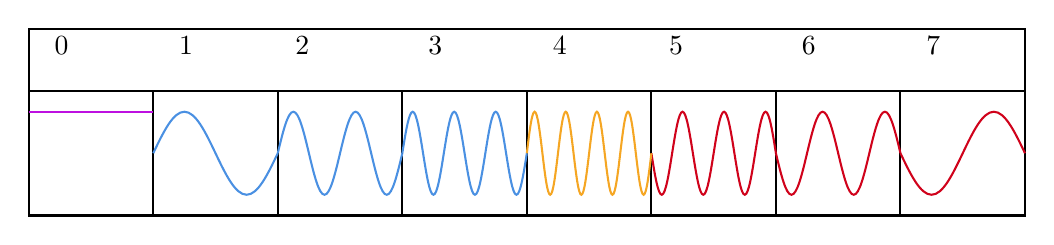
\begin{tikzpicture}[x=0.75pt,y=0.75pt,yscale=-1,xscale=1]
%uncomment if require: \path (0,300); %set diagram left start at 0, and has height of 300

%Shape: Rectangle [id:dp7496677292319892] 
\draw   (50,50) -- (530,50) -- (530,110) -- (50,110) -- cycle ;
%Straight Lines [id:da8481300844829959] 
\draw    (110,50) -- (110,110) ;
%Straight Lines [id:da9979873447579766] 
\draw    (170,50) -- (170,110) ;
%Straight Lines [id:da6604207247390047] 
\draw    (230,50) -- (230,110) ;
%Straight Lines [id:da17552724160417987] 
\draw    (290,50) -- (290,110) ;
%Straight Lines [id:da1001580277439017] 
\draw    (350,50) -- (350,110) ;
%Straight Lines [id:da1242292963278292] 
\draw    (410,50) -- (410,110) ;
%Straight Lines [id:da14184261120587927] 
\draw    (470,50) -- (470,110) ;
%Shape: Wave [id:dp7482546835654859] 
\draw  [color={rgb, 255:red, 74; green, 144; blue, 226 }  ,draw opacity=1 ] (110,80) .. controls (114.89,69.75) and (119.57,60) .. (125,60) .. controls (130.43,60) and (135.11,69.75) .. (140,80) .. controls (144.89,90.25) and (149.57,100) .. (155,100) .. controls (160.43,100) and (165.11,90.25) .. (170,80) ;
%Shape: Rectangle [id:dp19496511581663822] 
\draw   (50,20) -- (530,20) -- (530,50) -- (50,50) -- cycle ;
%Straight Lines [id:da9584443678032528] 
\draw [color={rgb, 255:red, 189; green, 16; blue, 224 }  ,draw opacity=1 ]   (50,60) -- (110,60) ;
%Shape: Wave [id:dp660538452942873] 
\draw  [color={rgb, 255:red, 74; green, 144; blue, 226 }  ,draw opacity=1 ] (170,80) .. controls (172.45,69.75) and (174.79,60) .. (177.5,60) .. controls (180.21,60) and (182.55,69.75) .. (185,80) .. controls (187.45,90.25) and (189.79,100) .. (192.5,100) .. controls (195.21,100) and (197.55,90.25) .. (200,80) .. controls (202.45,69.75) and (204.79,60) .. (207.5,60) .. controls (210.21,60) and (212.55,69.75) .. (215,80) .. controls (217.45,90.25) and (219.79,100) .. (222.5,100) .. controls (225.21,100) and (227.55,90.25) .. (230,80) ;
%Shape: Wave [id:dp9332879206435427] 
\draw  [color={rgb, 255:red, 74; green, 144; blue, 226 }  ,draw opacity=1 ] (230,80) .. controls (231.63,69.75) and (233.19,60) .. (235,60) .. controls (236.81,60) and (238.37,69.75) .. (240,80) .. controls (241.63,90.25) and (243.19,100) .. (245,100) .. controls (246.81,100) and (248.37,90.25) .. (250,80) .. controls (251.63,69.75) and (253.19,60) .. (255,60) .. controls (256.81,60) and (258.37,69.75) .. (260,80) .. controls (261.63,90.25) and (263.19,100) .. (265,100) .. controls (266.81,100) and (268.37,90.25) .. (270,80) .. controls (271.63,69.75) and (273.19,60) .. (275,60) .. controls (276.81,60) and (278.37,69.75) .. (280,80) .. controls (281.63,90.25) and (283.19,100) .. (285,100) .. controls (286.81,100) and (288.37,90.25) .. (290,80) ;
%Shape: Wave [id:dp7967792640311087] 
\draw  [color={rgb, 255:red, 208; green, 2; blue, 27 }  ,draw opacity=1 ] (350,80) .. controls (351.63,90.25) and (353.19,100) .. (355,100) .. controls (356.81,100) and (358.37,90.25) .. (360,80) .. controls (361.63,69.75) and (363.19,60) .. (365,60) .. controls (366.81,60) and (368.37,69.75) .. (370,80) .. controls (371.63,90.25) and (373.19,100) .. (375,100) .. controls (376.81,100) and (378.37,90.25) .. (380,80) .. controls (381.63,69.75) and (383.19,60) .. (385,60) .. controls (386.81,60) and (388.37,69.75) .. (390,80) .. controls (391.63,90.25) and (393.19,100) .. (395,100) .. controls (396.81,100) and (398.37,90.25) .. (400,80) .. controls (401.63,69.75) and (403.19,60) .. (405,60) .. controls (406.81,60) and (408.37,69.75) .. (410,80) ;
%Shape: Wave [id:dp026782774832921463] 
\draw  [color={rgb, 255:red, 208; green, 2; blue, 27 }  ,draw opacity=1 ] (410,80) .. controls (412.45,90.25) and (414.79,100) .. (417.5,100) .. controls (420.21,100) and (422.55,90.25) .. (425,80) .. controls (427.45,69.75) and (429.79,60) .. (432.5,60) .. controls (435.21,60) and (437.55,69.75) .. (440,80) .. controls (442.45,90.25) and (444.79,100) .. (447.5,100) .. controls (450.21,100) and (452.55,90.25) .. (455,80) .. controls (457.45,69.75) and (459.79,60) .. (462.5,60) .. controls (465.21,60) and (467.55,69.75) .. (470,80) ;
%Shape: Wave [id:dp36599669274032653] 
\draw  [color={rgb, 255:red, 208; green, 2; blue, 27 }  ,draw opacity=1 ] (470,80) .. controls (474.89,90.25) and (479.57,100) .. (485,100) .. controls (490.43,100) and (495.11,90.25) .. (500,80) .. controls (504.89,69.75) and (509.57,60) .. (515,60) .. controls (520.43,60) and (525.11,69.75) .. (530,80) ;
%Shape: Wave [id:dp378953214883782] 
\draw  [color={rgb, 255:red, 245; green, 166; blue, 35 }  ,draw opacity=1 ] (290,80) .. controls (291.22,69.75) and (292.39,60) .. (293.75,60) .. controls (295.11,60) and (296.28,69.75) .. (297.5,80) .. controls (298.72,90.25) and (299.89,100) .. (301.25,100) .. controls (302.61,100) and (303.78,90.25) .. (305,80) .. controls (306.22,69.75) and (307.39,60) .. (308.75,60) .. controls (310.11,60) and (311.28,69.75) .. (312.5,80) .. controls (313.72,90.25) and (314.89,100) .. (316.25,100) .. controls (317.61,100) and (318.78,90.25) .. (320,80) .. controls (321.22,69.75) and (322.39,60) .. (323.75,60) .. controls (325.11,60) and (326.28,69.75) .. (327.5,80) .. controls (328.72,90.25) and (329.89,100) .. (331.25,100) .. controls (332.61,100) and (333.78,90.25) .. (335,80) .. controls (336.22,69.75) and (337.39,60) .. (338.75,60) .. controls (340.11,60) and (341.28,69.75) .. (342.5,80) .. controls (343.72,90.25) and (344.89,100) .. (346.25,100) .. controls (347.61,100) and (348.78,90.25) .. (350,80) ;

% Text Node
\draw (61,22.4) node [anchor=north west][inner sep=0.75pt]    {$0$};
% Text Node
\draw (121,22.4) node [anchor=north west][inner sep=0.75pt]    {$1$};
% Text Node
\draw (177,22.4) node [anchor=north west][inner sep=0.75pt]    {$2$};
% Text Node
\draw (241,22.4) node [anchor=north west][inner sep=0.75pt]    {$3$};
% Text Node
\draw (301,22.4) node [anchor=north west][inner sep=0.75pt]    {$4$};
% Text Node
\draw (357,22.4) node [anchor=north west][inner sep=0.75pt]    {$5$};
% Text Node
\draw (421,22.4) node [anchor=north west][inner sep=0.75pt]    {$6$};
% Text Node
\draw (481,22.4) node [anchor=north west][inner sep=0.75pt]    {$7$};


\end{tikzpicture}
\end{center}

\subsection{Short time Fourier transform}
To analyse how the frequencies of a audio signal change over time, we can
divide the audio stream into overlapping \emph{windows} of samples.
The DFT is applied to each window, which gives information about the frequencies
present at that moment in time.

\begin{center}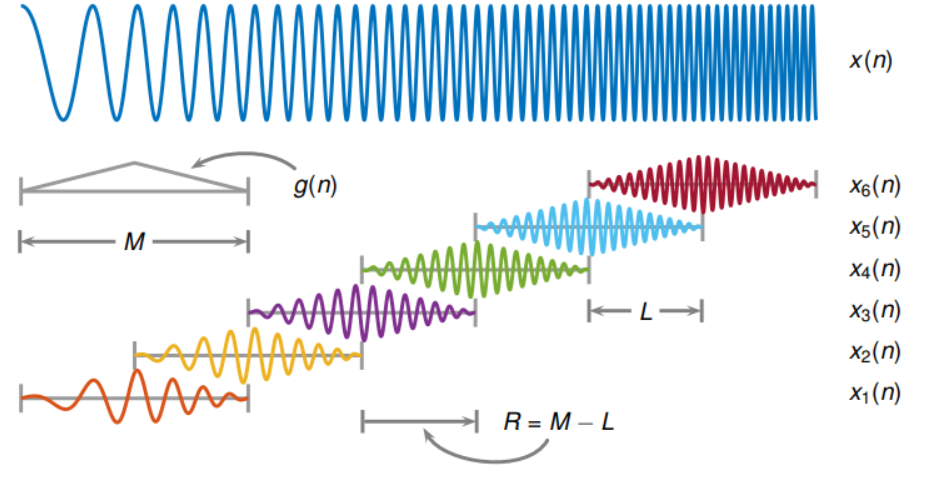
\includegraphics[height=5cm]{assets/windowing.png}\end{center}

For best results, a windowing function is applied to each window, in order
to taper the edges of the signal to zero to avoid discontinuities at the edges.

\pagebreak

\subsection{Spectrograms}
A spectrogram is a visual tool used to see what frequencies are present at 
each moment in time.
This information is represented as a heatmap, where the input variables are on the $x$ and $y$ axes,
and the magnitude of output is represented using colour/brightness.
In the example screenshot below, frequency (on the $y$-axis) is shown on a logarithmic scale.
Most spectrograms represent frequency on a log scale because humans perceive pitch logarithmically.

\begin{center}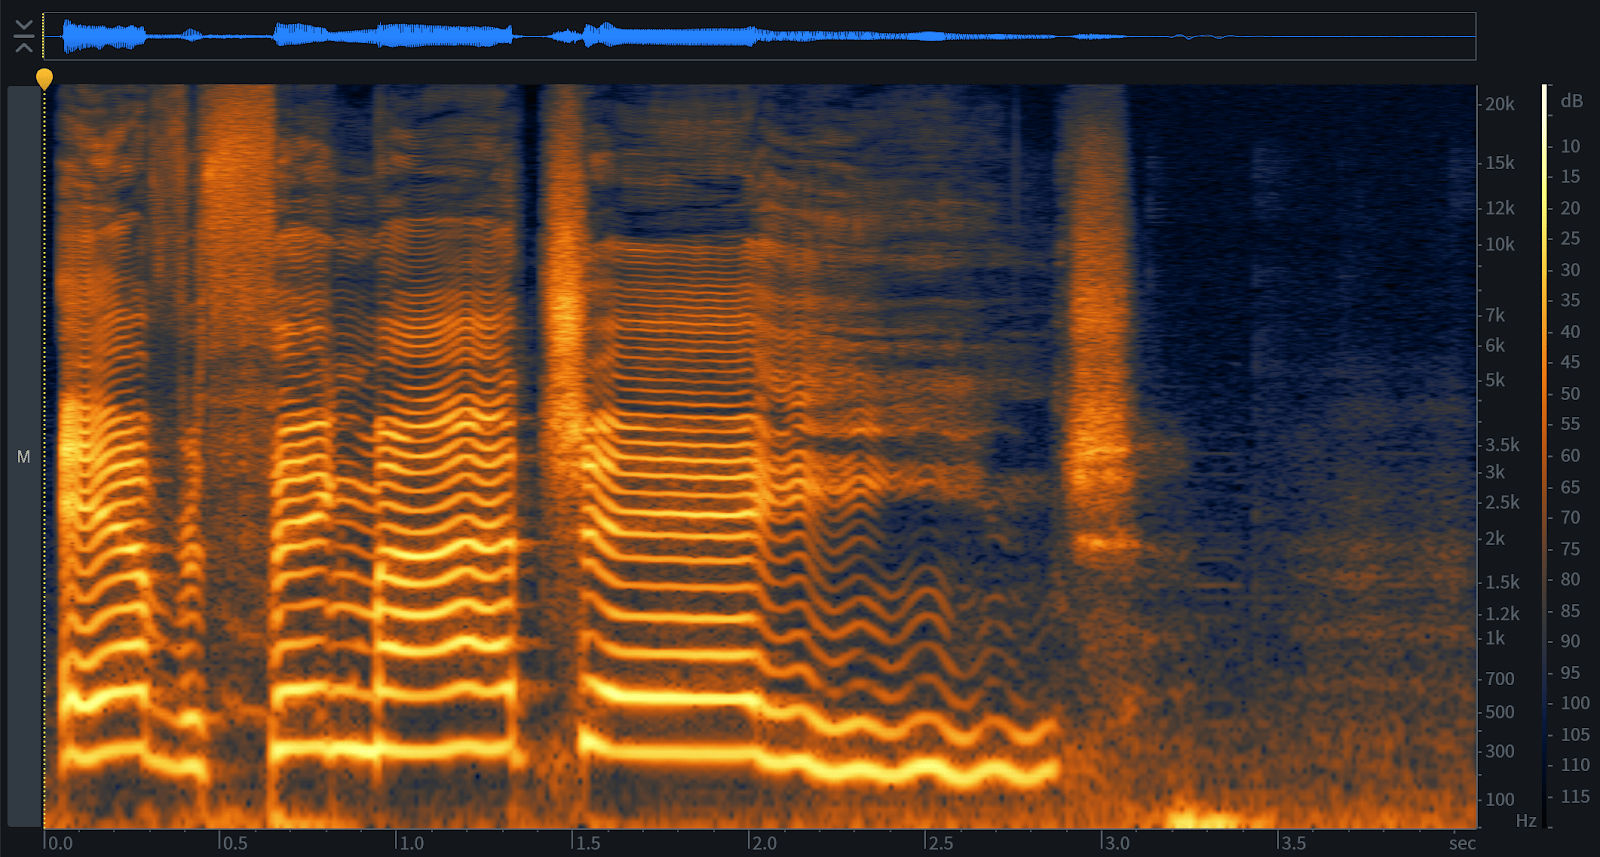
\includegraphics[height=6cm]{assets/spectrogram.jpg}\end{center}

It is a tool commonly used in electronic music production. 
It makes use of the STFT to determine the frequency composition of the signal
at each moment in time.

A setting that can be changed by the user is the FFT window size.
The size determines the frequency-resolution vs time-resolution tradeoff.
The wider the windows, the more frequency bins there are resulting in more 
frequency-resolution. However you will be capturing a larger portion of audio,
which wouldn't work well if the frequencies are changing quickly over time, resulting in 
reduced time-resolution (even if overlapping windows are used).

\begin{center}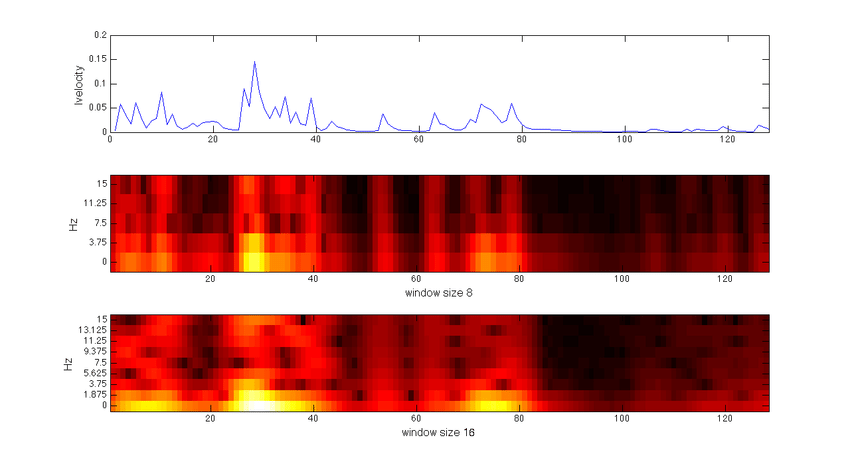
\includegraphics[height=9cm]{assets/resolution.png}\end{center}

